\documentclass[aps,pre,twocolumn,showpacs,amsmath,amssymb]{revtex4-1}

\usepackage{graphicx}
\usepackage{color}

\usepackage[portuguese]{babel}
\usepackage[utf8]{inputenc}
\usepackage[T1]{fontenc}

\usepackage{titlesec}

\titlespacing*{\section}{0pt}{\baselineskip}{\baselineskip}
\titlespacing*{\subsection}{0pt}{\baselineskip}{\baselineskip}

\hfuzz 1pt
\vfuzz 1pt

\setlength{\parskip}{\baselineskip}

\begin{document}

\title{Exercício 3: Otimização de Funções}
\author{Ernesto González, Cláudia Reis, Beatriz Araújo}

\begin{abstract}
%    Implementação e comparação da eficácia do método do Número de Ouro, do método do Gradiente e do método de Newton a encontrar extremos de funções e verificar a influência de certos parâmetros destes métodos no seu desempenho.

    Comparação da eficácia dos métodos do Número de Ouro, do Gradiente e de Newton na determinação de extremos de funções. Estudo do impacto de parâmetros destes métodos no seu desempenho. Impacto do "step" na convergência dos métodos e apresentação de técnicas para garanti-la.
\end{abstract}

\maketitle

\section{Corpo preso a uma mola}

\begin{figure}[h]\vspace{-5ex}
   \begin{center}
    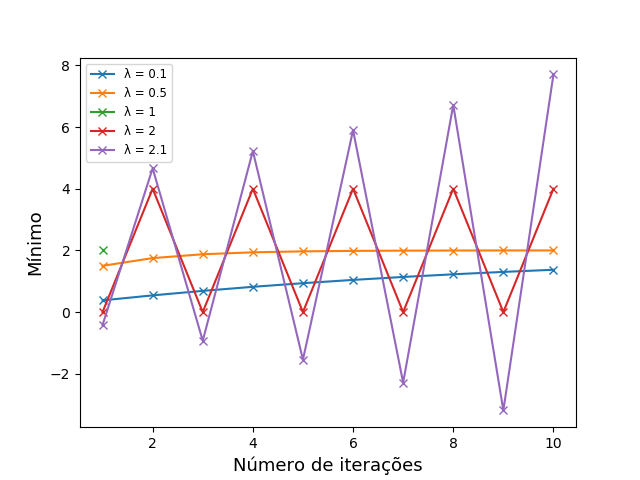
\includegraphics[width=\columnwidth]{1c.png} \\
\caption{Gráfico dos valores mínimos da função $0.5\cdot (x-2)^2$ em função do número de iterações pelo método do Gradiente para $x_0$ = 0 e $\lambda = 0.1$ (a azul), $\lambda = 0.5$ (a laranja), $\lambda = 1.0$ (a verde), $\lambda = 2.0$ (a vermelho) e $\lambda = 2.1$ (a roxo).}
   \end{center}
\end{figure}

O primeiro exercício tem como objetivo encontrar a posição de equilíbrio de um corpo que está sujeito a um potencial dado pela função $0.5\cdot (x-2)^2$. Para tal, implementámos dois métodos: o método do Número de Ouro ou método do Número Dourado e o método do Gradiente. \newline
\indent Primeiramente, implementou-se o método do Número de Ouro para os intervalos $a = [-0.7,2.6]$ e $b = [0.4, 1.7]$, com um critério de convergência de $0,001\%$, e obteve-se, respetivamente, $x_0 = 2.000004079290686$ e $x_0 = 1.6999835871019766$. Tendo em conta que o valor da posição de equibíbrio é $2.0$, conclui-se que o intervalo $b$ afastou-se um pouco do resultado em comparação com o intervalo $a$, isto porque o intervalo $b$ não contem o valor do potencial e, nesse caso, é dado o valor mais próximo possível dentro desse mesmo intervalo. \newline
\indent Posteriormente, foi implantado o método do Gradiente para a mesma função com os valores da constante $\lambda = [0.1; 0.5; 1.0; 2.0; 2.1]$, $x_0 = 0$, uma precisão de $1 \cdot 10^{-5}$ e um número máximo de iterações igual a $10$. \newline
\indent Para cada iteração, o $\it{Python}$ vai correr a expressão $x_{k+1} = x_k - \lambda f'(x_k)$ com $f'(x) = x - 2$ e, portanto, $f'(x_0) = - 2$. Logo, $x_1 = - 2\lambda$, $x_2 = 2\lambda - \lambda(2\lambda-2)$ e assim sucessivamente até $x_{k+a} - x_k < 1\cdot 10^{-5}$. \newline
\indent Observando a Figura 1, percebe-se que tanto $\lambda$ = 0.1 (a azul) como $\lambda = 0.5$ (a laranja) convergem para $x = 2$ por valores à esquerda deste, uma vez que, como $\lambda < 1$, $\lambda f'(x_k)$ tende para $0^+$ e $x_{k+1}$ tende para $2^-$. No entanto, como o número de iterações é limitado, para $\lambda = 0.1$ o método não consegue chegar ao valor pretendido usando apenas as 10 iterações, uma vez que o valor do $\lambda$ é demasiado pequeno o que faz com que haja uma convergência lenta. Isto já não acontece para $\lambda = 0.5$ que chega ao valor pretendido. Para $\lambda = 1$ (a verde), tem-se que $x_1 = x_2 = 2$ e, por isso, apresentar apenas esses dois pontos ($x_1$ corresponde à interação $0$). Para $\lambda = 2$ (a vermelho), $x_0 = 0$, $x_1 = 4$, $x_2 = 0$, e assim sucessivamente, pelo que, não havendo um limite de iterações, o método continuará infinitamente sempre entre $0$ e $4$. Para $\lambda = 2.1$ (a roxo) será algo semelhante, só que em vez de variar entre dois valores, irá estar sempre aumentar.


\section{Distância em ligação iónica - uma variável}

\indent \indent Estudou-se a função $U(r)=Ae^{-Br} - \frac{C}{r}$, que descreve o potencial de interação entre um ião $Na^+$ e um ião $Cl^-$, com os valores de A=80eV, C=10eVÅ, B=2Å$^{-1}$, de forma a encontrar a sua posiçao de equilíbrio, isto é, o ponto no qual o potencial é mínimo. \newline
\indent Com recurso ao Mathematica, representou-se graficamente a função $U(r)$ e calculou-se o seu mínimo usando a função FindMinimum (Fig. 2). Implementou-se também o método do Gradiente, em Python, com o valor inicial de $x_0=1$ para $\lambda=0.1$ e $\lambda=0.2$. Obteve-se $r=2.153299961768564$ com o FindMinimum, e $r=2.153321630545443$ com o método do Gradiente ($\lambda = 0.1$), o que indica que o último foi muito eficaz no apuramento do mínimo da função. \newline
\indent Implementou-se ainda o método de Newton para resolver o mesmo exercício. Este método é usado para determinar as raízes de uma função diferenciável. Neste caso, procura-se o mínimo da função $U$ que corresponderá a um ponto estacionário, isto é, um ponto no qual a derivada se anula. Portanto, aplicou-se este método à derivada da função, de forma a determinar as raízes de $U'(r)$. Obteve-se um mínimo em $r=2.1532923548433183$, valor muito próximo dos obtidos pelos dois métodos anteriores. \newline
\indent Comparou-se os métodos do Gradiente e de Newton (Figura 3). A diferença entre a eficácia dos métodos é notável, com o método de Newton a convergir mais rapidamente (apenas 6 iterações).
%"O método do gradiente vai evoluir na direção da maior taxa de decrescimento da função, ou seja otimiza (pelo estudo de U''(x)) a velocidade de convergência (dada por U'(x)) para o mínimo da função, daí ser mais rápido a convergir."

\begin{figure}[hbt!]\vspace{-7ex}
    \begin{center}
    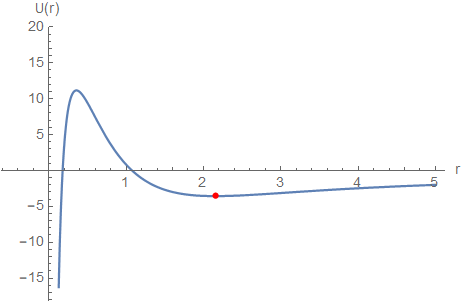
\includegraphics[width=\columnwidth]{2a.png}
    \caption{Potencial de interação ($U$) em função da distância entre os iões ($r$), para $r$ $\in$ $[0,5]$. A vermelho está representado o mínimo da função, calculado com o FindMinimum (Mathematica), com o valor $2.153299961768564$.}
    \end{center}
\end{figure}

\begin{figure}[hbt!]\vspace{-4ex}
    \begin{center}
    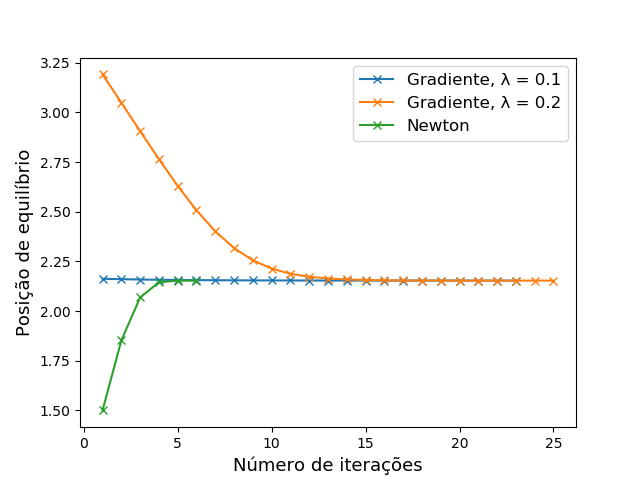
\includegraphics[width=\columnwidth]{2d_2.png}
    \caption{Posição de equilíbrio em função do número de iterações para o método do Gradiente, com $\lambda = 0.1$ (23 iterações) e $\lambda = 0.2$ (25 iterações), e para o método de Newton (6 iterações). Ambos com $x_0=1$.}
    \end{center}
\end{figure}

\section{Distância em ligação iónica - duas variáveis}
Consideremos agora $r=\sqrt{x^2+y^2}$. Da definição de $U(r)$, vem
$U(x,y)=80e^{-2\sqrt{x^2+y^2}}-\frac{10}{\sqrt{x^2+y^2}}.$\\
Encontra-se apresentado na Figura 2 o resultado da aplicação do método do gradiente 2D em $U(x,y)$ para $x_0=5$ e $y_0=-5$.
O mínimo encontrado pelo método do gradiente 2D, usando $\lambda=0.5$, é $(x,y)=(1.5226076382039215,-1.5226076382039215)$. É consistente com o mínimo $(x,y)=(1.52261,-1.52261)$ encontrado por FindMinimum do Mathematica.
Tendo em conta que $r=\sqrt{x^2+y^2}$, para o mínimo encontrado pelo gradiente 2D temos $r=\sqrt{(1.5226076382039215)^2+(-1.5226076382039215)^2}=2.153292372$, que é o mínimo encontrado para $U(r)$ usando o método do gradiente 1D na secção anterior, com um erro de $10^{-7}$. Outro aspecto interessante é como a trajetória seguida pelo método para chegar ao mínimo é $y=-x$. Isto deve-se à escolha do ponto de partida $(x_0,y_0)$, que no nosso caso respeita $y=-x$. Sendo que o gradiente segue uma trajetória radial na circunferência com centro em $(x,y)=(0,0)$ - como é de esperar pelas curvas de nível de circulares visíveis na Figura 5 - a trajetória seguida pelo método vai respeitar $y=\frac{y_0}{x_0}x$. A simetria das linhas de x por iteração e y por iteração em relação ao eixo das iterações deve-se também à simetria dos valores iniciais escolhidos.\\

Na Figura 5 vemos como o mínimo de $U(x,y)$ é em realidade uma circunferência de centro $(x,y)=(0,0)$ e raio entre $1.5$ e $3$, estando de acordo com o mínimo encontrado na secção anterior.

\begin{figure}[h]\vspace{-4ex}
   \begin{center}
    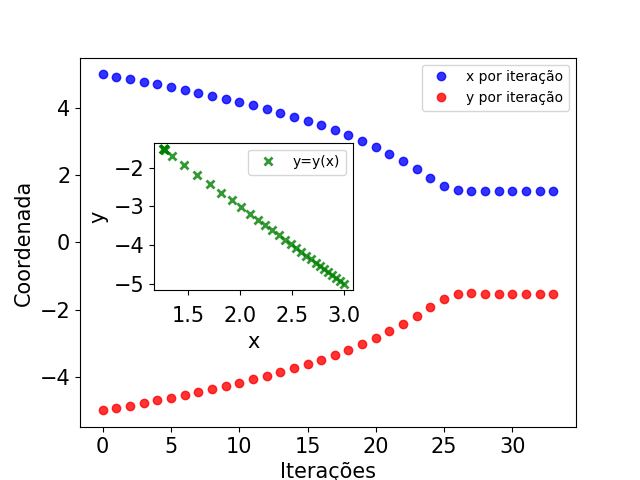
\includegraphics[width=\columnwidth]{potencialGradiente2D.png}
\caption{Resultados da aplicação do método do gradiente a $U(x,y)=80e^{-2\sqrt{x^2+y^2}}-\frac{10}{\sqrt{x^2+y^2}}$ para $\lambda=0.5$, partindo de $(x_0,y_0)=(5,-5)$. Os pontos azuis indicam o $x$ encontrado em cada iteração e os vermelhos o $y$. A linha verde indica o $y$ em função de x.}
  \label{potencialGradiente2D}
   \end{center}
\end{figure}

\begin{figure}[h]\vspace{0ex}
   \begin{center}
    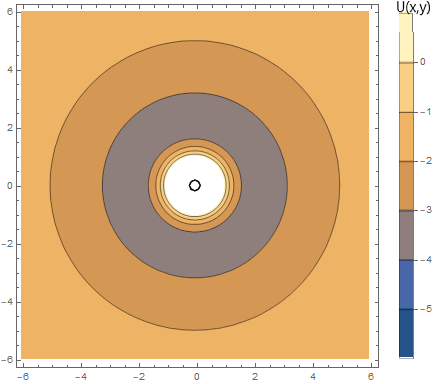
\includegraphics[width=\columnwidth]{potencial2DCurvasNivel.png}
\caption{Contour plot de $U(x,y)=80e^{-2\sqrt{x^2+y^2}}-\frac{10}{\sqrt{x^2+y^2}}$ com cada secção com potencial constante. A escala à direita indica o valor do potencial correspondente a cada cor.}
  \label{potencial2DCurvasNivel}
   \end{center}
\end{figure}

\section{Opcionais}

\subsection{Método da razão}
O método do número de ouro é uma variação do método da razão, em que a razão usada é $r=\frac{1+\sqrt{5}}{2}$. Na Figura 6 encontra-se o resultado da aplicação do método da razão para diferentes valores de $r$, aplicado para $[a,b]=[-0.7,2.6]$.
\begin{figure}[h]\vspace{-5ex}
   \begin{center}
    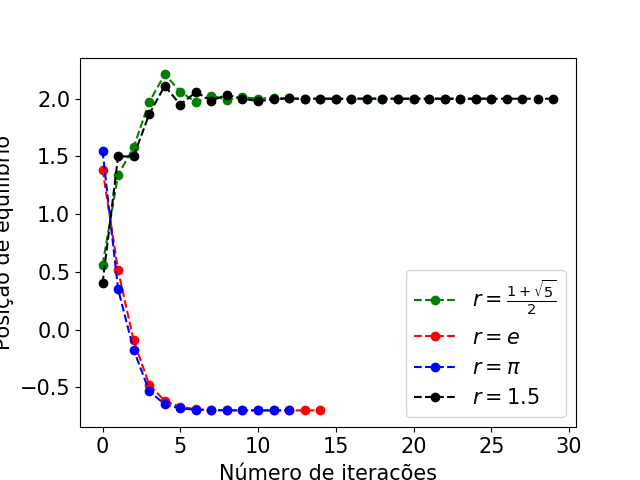
\includegraphics[width=\columnwidth]{ratiomethods.png}
\caption{Gráfico dos valores mínimos da função $0.5(x-2)^2$ em função do número de iterações pelo método da razão aplicado em $[a,b]=[-0.7,2.6]$ para diferentes valores de razão, $r$.}
  \label{ratiomethods}
   \end{center}
\end{figure}

\subsection{Optimização de $\lambda$ no método do gradiente}
Na secção I implementou-se o método do gradiente à função $0.5(x-2)^2$ para diferentes valores de $\lambda$ (ver Figura 1). Mencionou-se a importância da escolha do $\lambda$ na convergência do método. Consideremos agora o método do gradiente com optimização de $\lambda$, em que se fornece um $\lambda$ inicial, $\lambda_0$, e com $\lambda$ na n-ésima iteração dado por $\lambda_n=\frac{|(x_n-x_{n-1})(f'(x_n)-f'(x_{n-1}))|}{(f'(x_n)-f'(x_{n-1}))^2}$\footnote{Barzilai, Jonathan; Borwein, Jonathan M. (1988). "Two-Point Step Size Gradient Methods". IMA Journal of Numerical Analysis. 8 (1): 141–148.} - método do gradiente Barzilai-Borwein. Encontra-se na Figura 7 o resultado do método do gradiente simples para $\lambda=2.1$ e o método Barzilai-Borwein para $\lambda_0=2.1$

\begin{figure}[h]\vspace{0ex}
   \begin{center}
    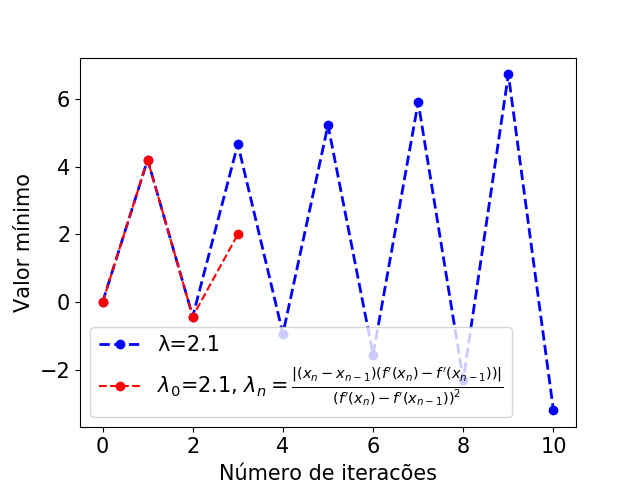
\includegraphics[width=\columnwidth]{otimizacaometodogradiente.png}
\caption{Gráfico dos valores mínimos da função $0.5(x-2)^2$ em função do número de iterações encontrados pelo método do gradiente para $x_0 = 0$ e $\lambda = 2.1$ (azul) e pelo método do gradiente Barzilai-Borwein para $x_0 = 0$ e $\lambda_0 = 2.1$ (vermelho).}
  \label{otimizacaometodogradiente}
   \end{center}
\end{figure}

Nas secções II e III consideramos o potencial de interação iónica em uma e duas dimensões. Considerando $U(x,y,z)=80e^{-2\sqrt{x^2+y^2+z^2}}-\frac{10}{\sqrt{x^2+y^+z^2}}$ aplicamos o método do gradiente 3D com $(x_0,y_0,z_0)=(5,-5,5)$ e obtivemos $(x,y,z)\approx(1.9031056,-0.783340,0.783340)$. Fazendo $r=\sqrt{x^2+y^2+z^2}$ obtemos $r=2.202057121870936$, assemelhando-se aos valores encontrados nos casos unidimensional e bidimensional.

\end{document}
